%\documentclass[aip, jcp, preprint]
\documentclass{article}[12pt]
\usepackage{graphicx}
\usepackage{amsmath}
\usepackage[margin=1in]{geometry}
\usepackage{color}

\title{Contributor Data Exploration at IndieGoGo}
\author{Ryan Applegate}
\begin{document}

\maketitle

\section{Data Exploration}

I explore a small sample of contribution data from IndieGoGo using minimal Python
scripts in the iPython notebook environment.

The data file is placed in a Pandas DataFrame for the majority of the analysis. My
first step is to take a quick look at the cateogories in each column of the data frame.
There are many contributors, campaigns, and perk ids, of similar magnitude as the total
number of records in the data set. These therefore are somewhat unsuitable for group
analysis as there are only a handful of points in each subset. That said, there are four
currencies, ninety-eight campaign countries and fifty contributor countries. These proved
to be somewhat suitable for some group level  statistics.


Globally, one can quickly find the mean and standard deviation using the "describe" method
in Pandas. I note however that I restrict my global analysis to USD currency, so that
transaction amounts can be combined sensibibly. For USD, the mean transaction amount is 78.78USD
and the std is 243.24 USD. Looking at only USD records accounts for ~88\% of the data.

\section{Claimed and Unclaimed Perks}

Each record has an optional field reporting if a "perk" was claimed by the contributor.
A non-NaN value means that the transaction amount exceeds some minimal perk amount, usually
resulting in the contributor getting some benefit. To attempt to understand what effect, if
any, claiming perks has on contributions, I plot a histogram of the number of transactions that
fall into a transaction amount bin. The interesting thing I observe is that there are "favored
values" which are usually "round numbers", i.e. 10, 50, 100 etc. (See attached html for images)

Presumably this clustering around nice numbers could come from either an incentive structure
in the perk amounts, or some human behavior aspect to gravitate toward "nice numbers". I attempt
to further investigate if the perk structure plays a role by plotting a histogram of the perk
amounts. There is the same underlying favoring of roung numbers in the histogram of perk
amounts, but this does not really tell us if they are driving the contribution distrubtion.

I plot another histogram, this time of contributions where a perk was not claimed (an unclaimed perk), hoping that the favoring of round numbers would not be as prevalent, but it is. Since
the structure toward nice numbers appears with and without the presence of claimed perks, I
am not able to say what effect perks incentivize users to spend in certain amounts.

\noindent
I can look at the distrubtions of the two groups, claimed and unclaimed, and note differnces in
the distrubtions. Both have similar means (~78USD and ~80USD) but different std (189USD and 335
USD), respectively. I next look at the difference in various quantiles( at the 25, 50 and 75 levels), and see that many more contributions occur at lower transaction amounts in the no
claimed case. 

\begin{verbatim}

                      Claimed Perk Unclaimed Perk
up to q 25%
    Total (USD)       21156        4826
    Per Contribution  12.21        6.67
    Percent Total     4.4%         2.2%
up to q 50%
    Total (USD)       59582        21328
    Per Contribution  18.86        14.36
    Percent Total     12.4%        9.9%
up to q 75%
    Total (USD)       137592       45312
    Per Contribution  29.89        22.53
    Percent Total     28.7%        21.1%

\end{verbatim}

This is actionable. If one could convert or incentivize contributors to behave as in the
claimed perk case, then more contributions would occur at the higher "per contribution"
values that appear when perks are claimed. The total percent increase in contrubtions
would look roughly as follows in the list below.

\begin{verbatim}
quantile    contribution increase    percent of all contribution increase
   q=25%       4005.29 USD               0.58%
   q=50%       6671.77 USD               0.96%
   q=75%       14800.43 USD              2.13%
\end{verbatim}

\section{Peak Usage}
We now turn to {\em when} contributions happen and look for patterns. Using the transaction
time column, I can group together temporally conincident points and get an idea of
trends across various time scales. I provide plots for the usage per day broken down by hour,
the usage per week broken down by day. Additional plots for the whole set are provided in
attached html file.

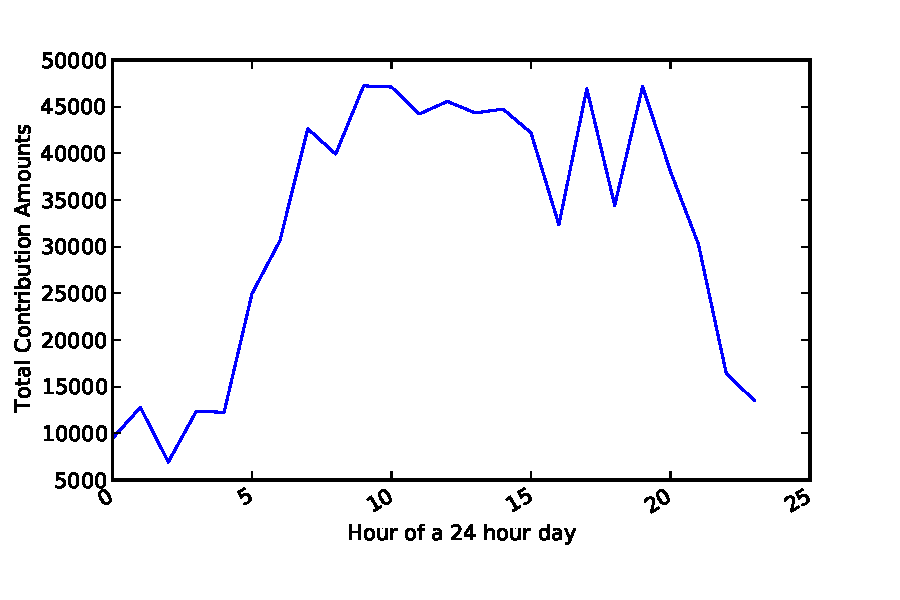
\includegraphics[scale=0.7]{Hours.pdf}

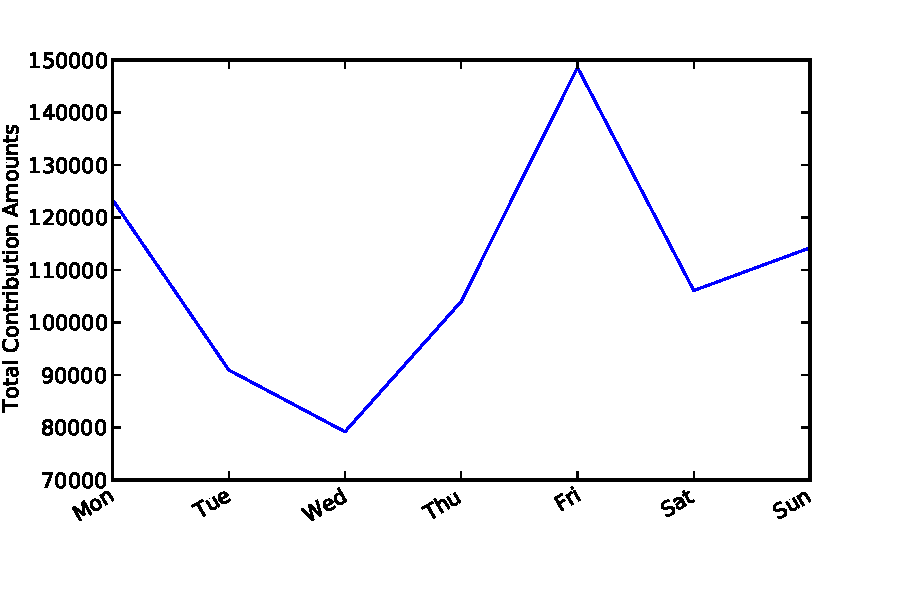
\includegraphics[scale=0.7]{DayOfWeek.pdf}

I conclude that most activity occurs between roughly 7AM and 6PM PST on an hourly basis.
 Additionaly, there is more activity on Fridays and to a lesser extent, over the weekend.
Both of these conclusions make sense, given we are looking at USD contributions and those are
mostly coming from continental US timezones.


\section{Conclusions}
Peak usage seems to be the clearest insight taken from the given dataset. In general, usage
can help with add targeting and user retention efforts by better understanding when people use
the site/service. Furthermore, usage can assist engineering efforts to assure that during peak
usage, no infrastructure is taxed to the point of a failure in quality service.

Perk structure is interesting, but the causal relationships are unclear given the short analysis here. On an indvidual contributor level, I would think there would be very clear
tendencies to try to reach perks on a regular basis. As there are minimal repeats of users
in this dataset, no such analysis can be even considered. However, I think specific analysis
on users and on the larger "genres" of campaigns they contribute to, would likely reveal some interesting patterns.


\end{document}
